% =============================================================================
% QIGOA Reality-Check — manuscript skeleton
% =============================================================================
% DISCIPLINE (CLAUDE.md §2, §5.3 · docs/preregistration.md §6 · docs/ke-hoach-trien-khai.md §3):
%
%   IRON RULE 1 — no invented numbers. Every quantity in this manuscript is
%                 either (a) \input{} from paper/tables/*.tex generated by
%                 scripts/build_tables.py out of results/*.csv, or (b) marked
%                 \PH / \TODO until such a table exists.
%   IRON RULE 2 — no invented citations. paper/refs.bib carries ONLY entries
%                 verified in docs/related-work-positioning.md. Entries whose
%                 given names / pages are not yet verified from a primary
%                 source carry an explicit % [VERIFY] comment there.
%   IRON RULE 3 — nothing is silently promoted from placeholder to result.
%
%   NUMBER FLOW IS ONE-WAY:  configs/ -> scripts/ -> results/ -> paper/
%   NEVER type a result number into any .tex file by hand.
%
% Formatting note: IEEEtran is used here because the writing standard for this
% project is the IEEE Transactions playbook (docs/lam-va-viet-paper-chuan-IEEE.md,
% mandated by CLAUDE.md §4). The target venue is BSPC (Elsevier); the class swap
% is a submission-time conversion (academic-paper skill), not a writing decision.
% =============================================================================

\documentclass[journal]{IEEEtran}

\usepackage{amsmath,amssymb,amsthm}
\usepackage{graphicx}
\usepackage{booktabs}
\usepackage{multirow}
\usepackage{url}
\usepackage[hidelinks]{hyperref}
\usepackage{xcolor}
\usepackage{tikz}
\usetikzlibrary{arrows.meta,positioning,fit,backgrounds}

\graphicspath{{figures/}}

% --- Placeholder machinery (IRON RULE 3) -------------------------------------
% \PH   : a number that does not exist yet. MUST NOT survive into submission.
% \TODO : prose that cannot be written until a result exists.
% Submission gate (ke-hoach §6): `grep -c 'PLACEHOLDER\|TODO' *.tex` must be 0.
\newcommand{\PH}{\textcolor{red}{\textbf{[PLACEHOLDER]}}}
\newcommand{\TODO}[1]{\textcolor{red}{[TODO: #1]}}

% Missing generated table/figure must not break the build while the pipeline
% has not run yet. When results/ is populated, these resolve automatically.
\newcommand{\inputtable}[1]{%
  \IfFileExists{tables/#1.tex}{\input{tables/#1.tex}}%
  {\centering\PH\\\footnotesize\texttt{tables/#1.tex} not generated yet.}}
\newcommand{\inputfigure}[2][\linewidth]{%
  \IfFileExists{figures/#2.pdf}{\includegraphics[width=#1]{#2.pdf}}%
  {\PH~\texttt{figures/#2.pdf} not generated yet.}}

% --- PREREGISTERED DESIGN CONSTANTS ------------------------------------------
% These are NOT results. Each is fixed a priori in docs/preregistration.md and
% is quoted here through a macro so the manuscript has exactly one source for
% it. Changing any of these means amending the preregistration first (§6,
% append-only) — never editing this block to match an outcome.
\newcommand{\kgrid}{\ensuremath{k \in \{2,3,4,5,6,8,10\}}}     % prereg §2
\newcommand{\kprimary}{\ensuremath{k=4}}                        % prereg §6/A4e
\newcommand{\sesoistrict}{\ensuremath{0.01}}                    % prereg §3 (Delta_1)
\newcommand{\sesoilenient}{\ensuremath{0.05}}                   % prereg §6/A4c (Delta_3)
\newcommand{\nsdtau}{\ensuremath{2}}                            % prereg §6/A7 (mm)
\newcommand{\nfolds}{five}                                      % prereg §6/A3
\newcommand{\graylevels}{\ensuremath{L=256}}                    % 8-bit histogram

\theoremstyle{plain}
\newtheorem{proposition}{Proposition}
\newtheorem{corollary}{Corollary}
\theoremstyle{definition}
\newtheorem{remark}{Remark}

\begin{document}

% =============================================================================
% TITLE — framing decision #1 (ke-hoach §4): neutral, descriptive, benchmark-
% shaped. The earlier working title "Optimizing the Wrong Variable" is BANNED:
% it guarantees a hostile associate editor from the metaheuristic community,
% which is the community the editor will draw reviewers from.
% =============================================================================
\title{Benchmarking Metaheuristic and Quantum-Inspired Multilevel Thresholding
for Brain Tumor Segmentation: An Exact-Optimum Reference, a Ceiling
Decomposition, and an Evaluation Protocol}

\author{\TODO{author block, affiliations, ORCID, funding --- fill at submission}}

\maketitle

% =============================================================================
% ABSTRACT — framing decision #2 (ke-hoach §4): OPEN WITH THE CONTRIBUTION,
% NOT WITH THE ACCUSATION. The critical finding appears at sentence 4--5 as an
% *empirical observation*, never as a verdict on named authors.
% Framing decision: Menotti (exact solver), Francois & Tinarrage (ceiling) and
% Hammouche (metaheuristics vs. global optimum) MUST be cited in the abstract —
% a paper whose thesis is "the field does not cite the exact solution" that
% fails to cite them self-immolates in one sentence.
% =============================================================================
\begin{abstract}
Multilevel thresholding driven by metaheuristic and quantum-inspired optimizers
remains an active line of work on medical images, yet the optimization problem
it attacks admits an exact polynomial-time solution~\cite{menotti_ciarp}, and
the segmentation quality attainable by any intensity threshold on brain MRI is
already known to be bounded~\cite{francois_jmiv}.
We contribute (i)~a ground-truth-anchored benchmark of metaheuristic, quantum-inspired
and random search under an exactly equal function-evaluation budget, referenced
against the exact global optimum rather than against one another, following the
protocol pioneered on gray-level images by Hammouche \emph{et al.}~\cite{hammouche_eaai};
(ii)~a \emph{decomposition} of the reported thresholding ceiling into the part
explained by the restriction to a contiguous intensity band, the part explained
by the restriction to intensity information at all, and the part recovered by a
learned model on identical input; and (iii)~an inexpensive diagnostic that
computes the attainable Dice of the entire thresholding family from an image
histogram, together with an evaluation-protocol checklist.
On $368$ patients of BraTS~2020, no metaheuristic reaches the exact optimum at a
$0.99$ hit rate for any threshold count, yet the per-patient Dice of every method
is statistically equivalent to that of the exact global optimum (median
difference zero; two one-sided tests pass at a $0.05$ margin in all $36$
comparisons): the optimization gap does not project onto the clinical mask.
Decomposing the achievable ceiling with a 2-D U-Net on identical single-slice
input places the residual shortfall in spatial structure rather than intensity,
the learned model exceeding the intensity-only ceiling by a median $0.050$ Dice
on whole tumor. We claim no quantum advantage, no speed record, and no new
ceiling.
Analyses were pre-specified in a confirmatory analysis protocol registered at
\TODO{OSF/Zenodo DOI --- prereg §6/A9, author task, before any real run};
code and seeds are public.
\end{abstract}

\begin{IEEEkeywords}
Multilevel thresholding, Kapur entropy, metaheuristics, quantum-inspired
optimization, brain tumor segmentation, evaluation methodology, dynamic
programming.
\end{IEEEkeywords}

% =============================================================================
% §1 INTRODUCTION
% WRITE THIS SECTION LAST (ke-hoach §4): reading order != writing order. §3 and
% §8 are the soul of the paper; the introduction can only be written once we
% know what the paper actually says.
%
% TONE (ke-hoach §4, framing): criticize PRACTICE, never name an author to
% disparage them. The editor draws reviewers from this community.
% =============================================================================
\section{Introduction}
\label{sec:intro}

% --- Frame: the line of work is alive, on medical images, into 2026 ----------
Multilevel thresholding remains one of the most widely used unsupervised
segmentation primitives, and the search for the threshold vector that maximizes
a criterion such as Kapur's entropy continues to be posed as an optimization
contest between population-based metaheuristics, including quantum-inspired
variants, on medical images~\cite{alnajdawi_scirep,mousavirad_kbs}.

% --- The two facts that reframe the contest, both already in print -----------
Two established results bracket that contest. First, the optimization problem
is not open: exact, polynomial-time dynamic programming for Kapur, Otsu and
Kittler--Illingworth criteria has been available for over a
decade~\cite{menotti_ciarp,luessi_jei,merzban_eswa}, and metaheuristics have
been benchmarked against a global optimum on gray-level images since at least
2010~\cite{hammouche_eaai}. Second, on brain MRI the segmentation quality
attainable by \emph{any} intensity threshold is bounded, and that bound has
been reported on BraTS FLAIR~\cite{francois_jmiv}.
% RED LINE (prereg §6/A2): never write "we establish the ceiling" — Francois &
% Tinarrage established it. We cite it as an established result.

What is missing is the projection between them: whether the optimization gap
these algorithms compete over survives the mapping onto a clinically scored
binary mask. That mapping is where ground truth enters, and it is exactly the
step that is absent from evaluations conducted in the objective's own units, or
on images without segmentation ground truth~\cite{mousavirad_kbs,hegazy_metricbias}.

\subsection{Contributions}
% Framing: contributions are a BENCHMARK + a TOOL + a PROTOCOL (CLAUDE.md §1).
% "Millisecond exact solver" is NOT a contribution — Menotti et al. published it
% eleven years ago. "We establish the ceiling" is NOT a contribution — Francois &
% Tinarrage published it. Anything resembling either must be deleted on sight.
\begin{enumerate}
  \item \textbf{A ground-truth-anchored benchmark under an exactly equal
  evaluation budget.} Every metaheuristic, the quantum-inspired variant and
  random search consume an identical, asserted number of objective function
  evaluations, and all are referenced against the \emph{exact} global optimum
  obtained by dynamic programming~\cite{menotti_ciarp} rather than against one
  another. Solutions are scored both in fitness units and in clinical Dice on
  BraTS whole-tumor masks.

  \item \textbf{A decomposition of the thresholding ceiling.} We separate the
  bound attainable by a contiguous-intensity-band mask, the bound attainable by
  an arbitrary gray-level set --- the tightest bound for any intensity-only
  decoder, obtained by applying the F1-threshold result of Lipton \emph{et
  al.}~\cite{lipton_f1} --- and the performance of a learned model on identical
  single-slice input. This separates the shortfall into ``information absent
  from intensity'' and ``information absent from the pixels.''
  % We claim the APPLICATION and the DECOMPOSITION, never the mathematics.

  \item \textbf{A histogram-time diagnostic and an evaluation-protocol
  checklist.} The attainable Dice of the entire thresholding family follows from
  the image histogram and the reference mask in $O(L \log L)$, i.e. before the
  first line of an optimizer is written.
\end{enumerate}

% --- Honest statement of what this paper is ---------------------------------
This is a benchmark and protocol paper: a reality check with a constructive
component, in the sense of a rigorously conducted negative finding paired with a
usable tool. \TODO{one sentence naming the empirical headline, once results/
exists --- phrased as an observation, never as a verdict.}

\TODO{closing paragraph: paper roadmap, written last.}

% =============================================================================
% §2 RELATED WORK & THE CITATION GAP
% Source of every paragraph below: docs/related-work-positioning.md (Week-0 gate,
% completed 16/07/2026). Those paragraphs were written as drop-in positioning
% text against VERIFIED metadata; do not paraphrase them into stronger claims.
%
% Related work = POSITIONING, not a list (playbook §6.5): lead with the
% integrated contribution, name and DISTINGUISH the near-rivals.
%
% ⚠️ FRAMING DECISION #3 (ke-hoach §4): the BIBLIOMETRIC table (N papers that do
% not cite an exact solution / do not measure Dice) goes to SUPPLEMENTARY. If
% the first table an editor sees is "we counted papers that failed to cite X",
% the paper is classified as meta-science and desk-rejected as out of scope.
% Table I of the manuscript is DP vs. exhaustive search (§3) — mathematics, not
% an accusation.
% =============================================================================
\section{Related Work and the Citation Gap}
\label{sec:related}

\subsection{Metaheuristic and Quantum-Inspired Multilevel Thresholding}

\TODO{2--3 paragraphs surveying the line of work, at the level of PRACTICE, not
of named authors. Cite from refs.bib only. Any count of papers ("N of M studies
report no Dice") comes from the coded bibliometric survey and may be stated only
once that survey exists with its two-coder Cohen's $\kappa$ --- see the
supplementary table and docs/RESULTS.md.}

% Recent, large, medical-image optimizer benchmark: the strongest checkable
% evidence for the thesis. Numbers in this paper's records are [PARTIAL] —
% re-open the full text before quoting any of them (positioning §7).
Al-Najdawi \emph{et al.}~\cite{alnajdawi_scirep} provide a large-scale, recent
benchmark of optimization algorithms coupled with Otsu's method on medical
images, reporting strong overlap scores while acknowledging in their limitations
the absence of ground-truth annotations. We treat this not as a competitor but
as evidence for the question we ask: the field continues to rank optimizers on
medical images by surrogate criteria. \TODO{quote their exact figures only after
re-opening the full text --- currently [PARTIAL], gated.}

% Positioning of the quantum-inspired branch.
% RED LINE (CLAUDE.md §1, lằn ranh 3): the words "quantum advantage", "quantum
% speedup", "quantum parallelism" are BANNED anywhere in this manuscript.
% Correct positioning: "an EDA-style probabilistic update rule", anchored to
% Platel et al., who showed QIEA is an EDA. Submission gate greps for this.
Quantum-inspired evolutionary algorithms are classical algorithms: their qubit
representation and rotation-gate update have been characterized as an
estimation-of-distribution update rule~\cite{platel_tevc}. We therefore describe
the quantum-inspired component throughout as an EDA-style probabilistic update
rule. No benefit arising from quantum computation is claimed or implied: such a
claim would require quantum hardware, which is not involved here, and the
algorithms studied are classical throughout.
% Phrased to avoid the literal banned string so the submission grep stays clean.

\subsection{The Exact Solution Already Exists}

% Drop-in paragraph, positioning §5. Cited in the ABSTRACT as well.
Exact, polynomial-time computation of optimal multilevel thresholds --- for
Otsu, Kapur, and Kittler--Illingworth criteria alike --- was given by Menotti
\emph{et al.}~\cite{menotti_ciarp}, with an $O((K-1)L^2)$ dynamic program.
Related exact formulations appear in Luessi \emph{et al.}~\cite{luessi_jei} and
Merzban and Elbayoumi~\cite{merzban_eswa}, the latter demonstrating that the
exact solver dominates metaheuristics for the Otsu criterion on natural images.
We claim \emph{no novelty} for the exact solver; it is the reference optimum
against which we benchmark. Nor do we claim novelty for benchmarking
metaheuristics against a global optimum: Hammouche \emph{et
al.}~\cite{hammouche_eaai} compared six metaheuristics against an exhaustive
% ⚠️ [PARTIAL] — the 1e-9 convergence criterion and their Tables 8--10 are
% recorded in docs/related-work-positioning.md §6 from an earlier full-text read;
% the metadata is [VERIFIED] but this number was NOT re-read from the publisher
% record. RE-OPEN THE FULL TEXT before submission, or drop the number and keep
% the qualitative statement.
global optimum, defining convergence as $|F - F_{\mathrm{opt}}| \le 10^{-9}$, a
stricter criterion than ours, sixteen years earlier. Two things distinguish our
study. First, those studies operate on gray-level images without clinical ground
truth, so a residual fitness gap cannot be projected onto a Dice-scored mask; we
make exactly that projection the primary endpoint. Second, Hammouche \emph{et
al.} already observe that some methods fail to reach the optimum for larger
threshold counts --- a finding we corroborate and reframe rather than contradict.

A dynamic-programming treatment that also \emph{selects} the number of
thresholds, including on medical images, has recently been given by Hegazy and
Gabr~\cite{hegazy_dp}. We claim novelty for neither the exact solver nor
data-driven selection of the threshold count; our use of dynamic programming is
purely as a reference optimum, and our treatment of the threshold count is to
measure what selecting it under surrogate criteria costs in clinical terms.

\subsection{Evaluation Standards for Segmentation}

Mousavirad \emph{et al.}~\cite{mousavirad_kbs} pose precisely our optimization
question --- whether population-based metaheuristics are effective for
multilevel thresholding --- but in a setting that structurally cannot detect the
phenomenon we study: the objective is Otsu between-class variance on natural
benchmark images without segmentation ground truth, so performance is measured
\emph{in the objective's own units}. They report that recent algorithms differ
substantially, some failing to reach the optimum.
% RECONCILIATION #1 (positioning §HOA GIAI #1) — this apparent contradiction
% with our equivalence prediction MUST be addressed here, not left for a
% reviewer to find. It is resolved by the axis of measurement, and it is turned
% into a testable result by the decoupling test (prereg §6/A4b, P2c).
Our contribution is orthogonal on two axes: we evaluate against an exact global
optimum rather than against each other, and we project every solution onto a
clinical binary mask with ground truth. A fitness gap that is real in variance
units need not survive that projection; whether it does is itself one of our
pre-specified tests, rather than an assumption.

Hegazy and Gabr~\cite{hegazy_metricbias} demonstrate, on natural images, that
PSNR and SSIM correlate systematically more with Otsu's objective than with
Kapur's, cautioning that reported gains may reflect this bias rather than
genuine improvements. Our corresponding analysis is a \emph{domain extension},
not an independent discovery: we move the argument to clinical ground truth on
brain MRI and add the threshold-count axis.

% RECONCILIATION #2 (positioning §HOA GIAI #2) — the ceiling belongs to
% Francois & Tinarrage. Stating this plainly, in Related Work, is the defense.
The claim that intensity thresholding has a performance ceiling on brain MRI is
not ours to make: François and Tinarrage~\cite{francois_jmiv} already report, on
BraTS FLAIR, an oracle best Dice of $0.83 \pm 0.18$, describing this explicitly
as an upper bound on the achievable performance within the considered
thresholding framework. We take this as an established result and make no claim
to establishing a ceiling; our contribution is its \emph{decomposition}
(§\ref{sec:ceiling}).
% The one quoted number in this manuscript that is NOT ours: it is a quotation
% from a [VERIFIED] full text (positioning §2), attributed in the same sentence.
% Everything else numeric must come from results/ via build_tables.py.

\subsection{The Gap}

\TODO{closing paragraph naming the gap in one sentence, written after §3 and
§8. It must be a statement about what has not been MEASURED, not a statement
about what other authors failed to do.}

% =============================================================================
% §3 THE DEGENERACY OF THE OBJECTIVE  ★ write this section FIRST (ke-hoach §4)
%
% 🔴 RED LINE A1 (prereg §6/A1 · CLAUDE.md lằn ranh 4) — READ BEFORE WRITING:
% It is FORBIDDEN to write "the literature decodes by the brightest class
% [refs]". That rule was NOT FOUND in the literature — it is our own old code.
% Attributing it to cited works is MISREPRESENTATION OF CITED WORK = violation
% of IRON RULE 2, which is worse than any rejection risk.
%   - Most papers in this line produce no binary mask and use no ground truth.
%   - The minority that report Dice decode via a downstream segmenter (region
%     growing / k-means + morphology / morphological reconstruction).
%   - Papers that do binarize DO NOT STATE THE RULE.
% => Write the DILEMMA (Horn 1 / Horn 2). Both horns convict; the paper does not
%    need to know which horn the literature is on.
%
% Also (prereg §6/A1): std(Dice) < 1e-12 is a UNIT TEST (tests/test_degeneracy.py),
% NOT a Result. It has no p-value and passes on random noise. Present the
% mechanism as a Proposition + 3-line proof + Corollary; the headline number is
% the CARDINALITY RATIO, which is arithmetic, not an experiment.
% =============================================================================
\section{The Degeneracy of the Objective}
\label{sec:degeneracy}

\subsection{Problem Statement}

\TODO{formal setup, playbook §3.3: image $I: \Omega \to \{0,\dots,L-1\}$ with
$\graylevels$; threshold vector $T = \{t_1 < \dots < t_k\}$ partitioning the
intensity range into $k+1$ classes; Kapur's entropy objective written out with
the $0\log 0$ convention stated explicitly; the decoding map $\mathcal{D}$ from
label map to binary mask stated as a separate, explicit object --- because the
whole point of this section is that the literature leaves $\mathcal{D}$
unstated.}

% ⚠️ Conventions must be DECLARED here and locked before running (prereg §6/A5c):
% the 0log0 convention; whether empty classes are admissible; how duplicate
% thresholds are repaired; and above all WHETHER THE INTENSITY-ZERO BACKGROUND
% IS COUNTED IN THE HISTOGRAM (skull-stripped slices are ~65% zeros; this single
% choice changes the optimal thresholds, the Dice, and every PSNR/SSIM number).
% Both variants are run and both are reported.

\subsection{A Checkable Observation}

% This — not the attribution — is the empirical claim, and it is falsifiable by
% the supplementary bibliometric survey (two coders, Cohen's kappa).
Across the studies we surveyed, we did not find an explicit statement of the map
from the reported $k$-threshold vector to the binary mask that is scored.
\TODO{state the survey counts and $\kappa$ once the coded survey exists;
provenance: docs/RESULTS.md, supplementary table.}

\subsection{The Dilemma}

Because that map is unstated, we treat both possibilities, which are exhaustive.

\begin{itemize}
  \item \textbf{Horn 1 --- decoding by a band mask.} If the mask is the set of
  pixels whose intensity falls in a contiguous band of classes, possibly followed
  by morphological post-processing or connected-component selection on that
  binary mask, then the mask depends on at most two of the $k$ thresholds, and
  the remaining thresholds are free variables with respect to the reported score.

  \item \textbf{Horn 2 --- decoding by a downstream segmenter.} If the mask is
  produced by a downstream segmenter operating on the label map (k-means,
  watershed, region growing, active contours), then the mask is produced by that
  segmenter, and the thresholding stage has not been ablated in the studies we
  surveyed; the causal claim that a better optimizer yields a better mask is
  then untested rather than false.
\end{itemize}

\TODO{one closing sentence stating that the paper measures both horns rather
than assuming either --- the decoder set in §\ref{sec:protocol} includes both
band-selection rules and label-map-consuming segmenters, precisely so that the
mechanism below can be falsified.}

\subsection{Mechanism Under Horn 1}

\begin{proposition}[Band-selection decoding is at most two-dimensional]
\label{prop:degeneracy}
\TODO{statement: for any decoding that selects a contiguous band of classes
$[c_a, c_b]$, the induced mask $M = \{p : t_a \le I(p) < t_{b+1}\}$ depends only
on the pair $(t_a, t_{b+1})$, for any $k$.}
\end{proposition}

\begin{proof}
\TODO{three lines. This is arithmetic, not an experiment.}
\end{proof}

\begin{corollary}[Cardinality of the reachable mask family]
\label{cor:cardinality}
\TODO{the set of masks reachable by ANY band-selection decoding on an $L$-level
image has cardinality at most $\binom{L-1}{2}$, independent of $k$, while the
threshold search space at a given $k$ is $\binom{L-2}{k}$. State the ratio; it is
computed by arithmetic from $\graylevels$ and the preregistered $k$ grid, not
measured, so it carries no provenance row --- but it must still be produced by
the build script, not typed.}
\end{corollary}

\begin{remark}
Proposition~\ref{prop:degeneracy} is a statement about the decoding map, not
about any author's algorithm. It says nothing about whether an optimizer works;
it says what the reported score can possibly depend on.
\end{remark}

\subsection{The Optimization Problem Is Not Open}

Kapur's entropy is additive over intervals, so the optimal threshold vector is
computable exactly by dynamic programming in $O((K-1)L^2)$; this is
established~\cite{menotti_ciarp}, with related exact
formulations in~\cite{luessi_jei,merzban_eswa}, and we claim no novelty for it.
% ⛔ "Millisecond exact solver" was REMOVED from our contributions: Menotti et al.
% published exact Kapur, O((K-1)L^2), <160 ms, eleven years ago (CLAUDE.md §1).
% ⛔ Do NOT report a wall-clock speedup ("~250x"): that was an artifact of a
% Python loop. The currency is NFE + complexity; wall-clock is secondary.
We use it solely as the reference optimum. \TODO{one sentence on why an exact
reference changes the meaning of every comparison in this literature: gaps become
absolute rather than relative.}

% --- TABLE I of the manuscript = DP vs. exhaustive (framing decision #3) ------
% Provenance ledger row: "Bảng II" in docs/RESULTS.md.
% results/exact/dp_vs_bruteforce.csv <- scripts/run_exact_check.py
%   --config configs/exp_main.yaml   -> paper/tables/tab_dp_vs_bruteforce.tex
%   via scripts/build_tables.py. DO NOT TYPE THESE NUMBERS.
\begin{table}[t]
  \caption{Exact dynamic programming versus exhaustive search on real BraTS
  slices. Agreement criterion is preregistered: $|f_{\mathrm{DP}} -
  f_{\mathrm{brute}}| \le 10^{-9}$ \emph{and} identical induced mask under
  canonicalized thresholds. \TODO{complete caption: n images, k values, units,
  hardware --- self-explanatory per playbook §6.4.}}
  \label{tab:dp_vs_brute}
  \centering
  \inputtable{table2_dp_vs_bruteforce}
\end{table}

Table~\ref{tab:dp_vs_brute} reports the verification of the reference optimum
against exhaustive search. \TODO{one factual sentence once the gate has run.
This gate is hard: if it fails, no other experiment in this paper is valid, and
the first debugging step is an audit of the histogram conventions above, not of
the dynamic program.}

% =============================================================================
% §4 EXPERIMENTAL PROTOCOL
% Every choice below is preregistered (docs/preregistration.md, §2/§3 + §6
% amendments). Nothing here may be decided after seeing a number; if a choice
% must change, amend the preregistration first (append-only) and say so here.
%
% Evaluation is a REFUTATION TEST (playbook §6.3): each experiment is designed
% so that, if our claim is wrong, the experiment shows it.
% =============================================================================
\section{Experimental Protocol}
\label{sec:protocol}

\subsection{Preregistration}

We call the protocol by its honest name: a confirmatory analysis protocol for
exploratory findings. The degeneracy and surrogate-metric observations were first
noticed on an earlier pipeline that carried a budget defect, a defective
baseline, and self-rolled metrics; every number from that pipeline is discarded
and none is reused here. What remains from it is a set of hypotheses, and the
protocol below pre-specifies their confirmatory re-analysis: the decision metric,
success threshold, and analysis for each claim were fixed, in an append-only
document, before the clean grid was run, so that no choice in this section could
be made after seeing a number. \TODO{author task at submission: cite the public
OSF/Zenodo registration DOI of that protocol document.}

\subsection{Data and Cohort}

We use the BraTS~2020 training collection, the only split with public
voxel-level ground truth. Each patient contributes a single two-dimensional
slice, chosen a priori as the slice of largest whole-tumor area, so that the
input given to the thresholding methods and to the learned baseline is identical.
The cohort is every patient for which that slice is defined: $368$ of the $369$
released cases, one case being excluded by the a priori tumor-slice criterion.
The cohort manifest, with a per-case checksum, is committed with the code.

% ⚠️ Never claim "state of the art on the BraTS leaderboard": the real test set
% is held out on Synapse. We use the training split and split it ourselves.
% ⚠️ A8: the LGG cohort may NOT be external — BraTS 2020 absorbed TCGA-LGG cases
% from the same collection. name_mapping.csv MUST be cross-checked and the
% overlap REPORTED AS A NUMBER before the words "external validation" are used.
We evaluate on the publicly annotated training split and construct our own
patient-level splits; we make no claim relating to the withheld BraTS test set.
Two targets are studied. The primary is whole tumor on FLAIR, the most favorable
case for the methods under audit: a single bright region that a contiguous
intensity band can plausibly capture. The hard target is enhancing tumor on
T1ce, a bright rim around a dark necrotic core, a shape no single contiguous
intensity band can represent. The argument is a fortiori: a limitation that
appears even on the favorable target is not an artifact of a poorly chosen case,
and the hard target shows where the representational limit is provable rather
than measured.

\subsection{Splits and Leakage Control}

% 🔴 A3: this subsection exists because the positive contribution was, as
% originally planned, train-on-test. Inside a paper that criticizes unsound
% comparison, that is the ONE error that gets rejected for INTEGRITY.
Splitting is at the \textbf{patient} level, never the slice level.
\nfolds-fold outer cross-validation, stratified by grade and tumor-volume
tertile, with an inner validation fold inside each outer-training fold for
epoch selection. Methods are classified once, a priori, into three families and
evaluated accordingly:

\begin{itemize}
  \item \textbf{Family A --- unsupervised per-image methods}: the classical
  thresholds (Otsu, Li, triangle), $k$-means and GMM clustering, the exact
  dynamic program, the metaheuristics, and random search. These have no fitted
  parameters and are evaluated on every patient.
  \item \textbf{Family B --- methods with learned parameters}: the 2-D U-Net,
  the single-parameter percentile threshold, and any data-driven selection of the
  threshold count $k$. These are evaluated \emph{out-of-fold only}; scoring them
  on patients used to fit them would be the exact error this paper documents.
  \item \textbf{Family C --- oracles}: the contiguous-band and gray-level-set
  oracles. These are not methods but unattainable upper bounds; they consume the
  test-time ground truth and are labeled ``uses test-time ground truth'' in every
  table and figure.
\end{itemize}

Nested cross-validation yields exactly one out-of-fold value per patient for
every method, on the same patient set, which is what makes paired Wilcoxon,
Friedman, and equivalence testing well defined at all. Intensity normalization
is computed per image; dataset-level statistics would leak through preprocessing.
The ``identical input'' constraint on the learned baseline is a constraint at
\emph{inference}: the network is trained on the tumor-bearing slices of the
outer-training patients and evaluated on the single designated slice of each
held-out patient.

\subsection{Budget}

All metaheuristics, including the quantum-inspired variant and random search,
receive an identical hard budget of objective function evaluations. Every
evaluation passes through a single gate, so that opposition-based
initialization, Lévy steps and memetic refinement are counted; an assertion
requires each algorithm to consume exactly the same number of evaluations,
and the grid is void if it fails.
% This is the module that killed the earlier batch (a 13.4% budget surplus).
% tests/test_nfe_budget.py is a HARD GATE: fail => the grid must not run.
% Equal TUNING budget too, not just equal NFE (prereg §6/A6): apparent advantage
% in this field almost always comes from uneven tuning.

% A6: breaking the circularity. We must not label an implementation "broken"
% because it fails to reach the optimum — that is the very hypothesis under test.
Implementation correctness is established \emph{independently} of the
thresholding hypothesis: every implementation must first reproduce published
multilevel-threshold benchmark tables on standard gray-level images at the
published evaluation budget. Exclusion is by this a priori criterion only, and
excluded implementations are reported separately rather than dropped.

\subsection{Metrics}

The clinical endpoints are Dice and the 95th-percentile Hausdorff distance,
with the Normalized Surface Dice at tolerance $\nsdtau$~mm as primary and a
sensitivity analysis over $\{1,3,5\}$~mm; overlap and surface metrics use a named
public implementation, since a paper auditing evaluation may not rely on an
unnamed or self-rolled one. PSNR and SSIM are computed from a standard library
and reported as evidence about the surrogate criteria, never as quality results.
We also report the connected-component count of the predicted mask and the
empty-mask rate as an independent result. IoU is omitted as a monotone bijection
of Dice. Because Dice is bounded and skewed, it is summarized by its median with
interquartile range and a bootstrap confidence interval, not by mean and standard
deviation, and the per-patient distribution is provided.

% A7 conventions, locked before running:
% - empty predicted mask with non-empty GT => Dice 0, HD95 = declared fixed
%   penalty (image diagonal). Both empty => Dice 1, HD95 0.
% - 🔴 It is FORBIDDEN to silently drop empty-mask cases from HD95 statistics:
%   that is selection bias favoring thresholding exactly at large k.
% - mean±std is the WRONG summary for Dice (bounded, skewed, often bimodal):
%   report median [IQR] + bootstrap CI + the per-patient distribution.

\subsection{Statistics}

Paired comparisons use the Wilcoxon signed-rank test at the patient level with a
rank-biserial effect size; omnibus ranking uses Friedman with a Nemenyi
critical-difference diagram~\cite{demsar_cd}. Equivalence is tested by two
one-sided tests and reported as a $90\%$ confidence interval of the paired
difference together with the smallest margin at which equivalence holds, so that
the analysis returns a number rather than a pass/fail verdict; a Bayesian
signed-rank test with a region of practical equivalence is the primary
equivalence analysis~\cite{benavoli_bayes}. We state a SESOI hierarchy
($\sesoistrict$ strict, an inter-rater-anchored intermediate
bound~\cite{menze_brats}, and $\sesoilenient$ lenient) and report all three.
Multiple-testing families are declared explicitly; the intersection--union
equivalence tests are not corrected. The primary threshold count is $\kprimary$,
the primary decoding rule is band selection of the brightest class, and the
reference for equivalence is the exact dynamic program.

% 🔴 A4d — THE scipy TRAP. Under the degeneracy mechanism, two algorithms that
% find the same threshold produce bit-identical masks => paired difference is
% EXACTLY 0. scipy.stats.wilcoxon defaults to zero_method='wilcox', which DROPS
% all zero pairs: effective n collapses, and the test silently becomes a
% statement about the minority of patients where the algorithms disagree — the
% opposite of the paper's message, and a manufactured "significance" of exactly
% the kind this paper documents.
% LOCKED: zero_method='pratt', and report n_zero/n_total in EVERY paired table.
Tied pairs are handled by Pratt's method rather than being discarded, and the
number of exactly tied patients is reported in every paired comparison; under
the mechanism of §\ref{sec:degeneracy} such ties are the expected outcome, not a
nuisance.

% --- FIGURE 1 — pipeline + budget diagram (drawio-skill, manual) -------------
% Provenance: docs/RESULTS.md "Hình 1". Flow figures are drawn, not bitmapped
% (playbook §6.4).
\begin{figure}[t]
  \centering
  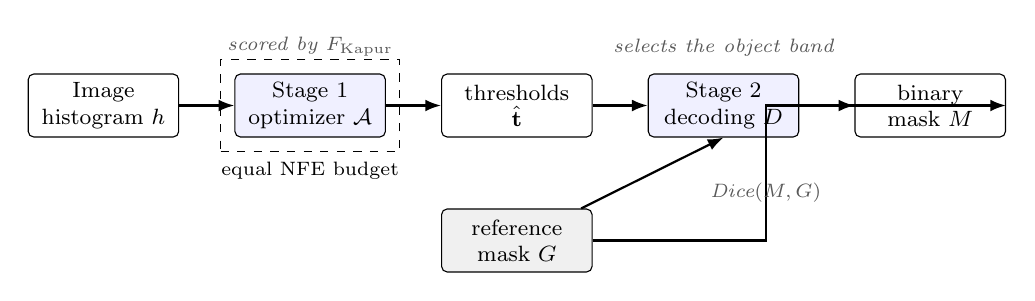
\begin{tikzpicture}[
    font=\footnotesize,
    node distance=6mm and 7mm,
    box/.style={draw, rounded corners=2pt, align=center, inner sep=3pt,
                minimum height=8mm, text width=17mm},
    stage/.style={box, fill=blue!6},
    oracle/.style={box, fill=gray!12},
    score/.style={align=center, font=\scriptsize\itshape, text=black!65},
    arr/.style={-{Latex[length=2mm]}, thick}]
    \node[box] (hist) {Image\\ histogram $h$};
    \node[stage, right=of hist] (opt) {Stage 1\\ optimizer $\mathcal{A}$};
    \node[box, right=of opt] (thr) {thresholds\\ $\hat{\mathbf t}$};
    \node[stage, right=of thr] (dec) {Stage 2\\ decoding $D$};
    \node[box, right=of dec] (mask) {binary\\ mask $M$};
    \node[oracle, below=9mm of thr] (gt) {reference\\ mask $G$};
    \draw[arr] (hist) -- (opt);
    \draw[arr] (opt) -- (thr);
    \draw[arr] (thr) -- (dec);
    \draw[arr] (dec) -- (mask);
    \draw[arr] (gt) -- (dec.south);
    \draw[arr] (gt.east) -- ++(2.2,0) |- (mask.east)
          node[pos=0.25, below, score]{Dice$(M,G)$};
    \node[score, above=1mm of opt] {scored by $F_{\mathrm{Kapur}}$};
    \node[score, above=1mm of dec] {selects the object band};
    % budget gate on the optimizer
    \node[draw, dashed, fit=(opt), inner sep=5pt, label={[font=\scriptsize]below:%
      equal NFE budget}] {};
  \end{tikzpicture}
  \caption{The two-stage pipeline. Stage~1 optimizes the threshold vector on the
  histogram and is scored in fitness units ($F_{\mathrm{Kapur}}$); Stage~2 decodes
  the intensity bands into a binary mask and is the only stage scored against the
  reference mask (Dice). A decade of work optimizes Stage~1. Every optimizer
  passes through a single evaluation gate enforcing an identical function-%
  evaluation budget. The reference mask enters only at Stage~2 and at scoring;
  fitting of any learned component is confined to the training split
  (§\ref{sec:protocol}).}
  \label{fig:pipeline}
\end{figure}

% =============================================================================
% §5 R1 — THERE IS NOTHING LEFT TO OPTIMIZE
% ⚠️ SCOPE (CLAUDE.md §1, ke-hoach §4): this proposition is DOWNGRADED to a
% short, citation-backed setup section. Menotti (exact solver), Hammouche
% (metaheuristics vs. exhaustive optimum, |F-F_opt|<=1e-9) and Merzban (exact DP
% beats metaheuristics) took nearly all of it. The only live piece is the
% equal-NFE comparison INCLUDING RANDOM SEARCH, and the projection onto Dice.
%
% ⚠️ Cost is reported as NFE + complexity. NOT wall-clock. The "~250x faster"
% claim is BANNED (Python-loop artifact, never measured).
% ⚠️ A6: an algorithm that misses the optimum is NOT evidence of a bug; the
% independent implementation gate (§4) decides that, not this result.
% ⚠️ Graded fallback (A4b): report k*, the largest k at which every algorithm
% reaches the optimum. If k* < max k, the preregistered sentence is that the
% algorithms fall short only where, by §3, the mask no longer changes — a
% STRONGER result, not a failure.
% NO RESULTS PROSE until results/main/summary.csv exists.
% =============================================================================
\section{The Optimization Gap}
\label{sec:r1}

\TODO{2 paragraphs of setup, citation-backed: that this comparison has been run
before on gray-level images~\cite{hammouche_eaai,merzban_eswa} and that we claim
no novelty for it; what is new here is (i) random search at an identical budget
and (ii) the projection of the fitness gap onto a clinically scored mask.}

% --- TABLE — gap to optimum, hit rate, NFE (provenance ledger: "Bảng III") ---
% results/main/summary.csv <- scripts/run_main_grid.py --config configs/exp_main.yaml
%   -> paper/tables/tab_main_grid.tex via scripts/build_tables.py, seeds {0..4}.
% Report median [IQR] + bootstrap CI (A7), NOT mean±std, for Dice columns.
\begin{table*}[t]
  \caption{Relative fitness gap to the exact optimum, hit rate, and consumed
  function evaluations, per algorithm and threshold count. \TODO{complete
  caption: n patients, seeds, budget, the equal-NFE assertion, and the fact that
  every algorithm consumed exactly the same budget.}}
  \label{tab:main_grid}
  \centering
  \inputtable{tab_main_grid}
\end{table*}

\TODO{results prose --- forbidden until the grid has run and its provenance row
in docs/RESULTS.md is filled.}

% --- FIGURE 2 — critical difference diagram ---------------------------------
% results/stats/cd.csv <- scripts/run_stats.py -> figures/fig2_cd.pdf
\begin{figure}[t]
  \centering
  \inputfigure{fig2_cd}
  \caption{Critical-difference diagram over patients~\cite{demsar_cd}.
  \TODO{caption: metric, n, seeds, post-hoc test.}}
  \label{fig:cd}
\end{figure}

\subsection{Decoupling Fitness from the Clinical Score}

% P2c (prereg §6/A4b): 5 lines of code, fully falsifiable, and it converts the
% "circularity" objection from a hole into a RESULT.
% Prediction, declared in advance: the correlation is approximately zero.
% If it is strong and positive, fitness IS a good proxy for Dice and the whole
% Goodhart argument weakens — that is what makes this a test rather than a demo.
We pre-specified a decoupling test: the rank correlation between an algorithm's
residual fitness gap and the magnitude of its Dice difference from the exact
solution. \TODO{report the coefficient and CI once available; state the
preregistered prediction and whether it survived. If the correlation is strong
and positive, the surrogate is a good proxy and we say so.}

\subsection{Mask Identity}

% The headline that needs no test: X% of (patient, k) cells where all algorithms
% emit BYTE-IDENTICAL masks. Report n_zero/n_total everywhere (A4d).
\TODO{report the fraction of (patient, threshold-count) cells on which the
compared algorithms produce byte-identical binary masks. This is a count, not an
inference; it requires no statistical test and admits no rebuttal. Source:
results/main/raw.csv via build\_tables.py.}

% =============================================================================
% §6 R2 — SURROGATE CRITERIA AND THE CLINICAL SCORE DISAGREE ALONG k
% ⚠️ POSITIONING (CLAUDE.md §1, P3): this is a DOMAIN EXTENSION of Hegazy & Gabr
% (metric bias, natural images) and a confirmation of the future work THEY
% themselves declare. It is NOT an independent discovery. Fardo et al. (2016)
% already covered PSNR-as-segmentation-metric including the k axis.
%
% ⚠️ A4a: the old decision rule (rho < -0.5 AND p < 0.05 over 7 values of k) is
% mathematically self-contradictory (critical |rho| ~ 0.786 at n=7) and rank
% correlation is the WRONG instrument for an inverted-U relationship. Averaging
% over k before correlating is an aggregation fallacy that HIDES the very
% Simpson's paradox this section is about.
% PRIMARY (locked): per-patient Delta_i = Dice_i(k*_Dice) - Dice_i(k*_PSNR),
% one-sample Wilcoxon over patients, rank-biserial + BCa bootstrap CI.
% The headline is a COST WITH CLINICAL UNITS, not a correlation coefficient.
%
% ⚠️ MANDATORY HONESTY (prereg §1/P3): within a FIXED k, the PSNR-Dice
% correlation across algorithms is POSITIVE. This must be stated by us, in this
% section. A reviewer reproduces it in ten minutes; concealing it kills the paper.
% NO RESULTS PROSE until results/main/summary.csv exists.
% =============================================================================
\section{Surrogate Criteria Along the Threshold-Count Axis}
\label{sec:r2}

\TODO{setup paragraph: credit Hegazy \& Gabr~\cite{hegazy_metricbias} for
establishing surrogate-metric bias on natural images and state plainly that this
section extends the question to clinical ground truth and to the threshold-count
axis; we claim the extension, not the discovery.}

\subsection{An Analytic Argument, Not Only a Correlation}

% Prove it, don't correlate it (A4a): PSNR is a monotone function of the
% quantization error, so it increases with k BY CONSTRUCTION (Lloyd-Max). An
% analytic argument cannot be defeated by sample size.
\TODO{short analytic argument that reconstruction-error-based surrogates
increase with the number of thresholds by construction, independently of any
segmentation quality. This is the part of the section that no sample size can
attack.}

\subsection{The Cost of Selecting the Threshold Count by a Surrogate}

% ⚠️ Selecting k is a LEARNED choice (prereg §6/A3, family B) => it may ONLY be
% evaluated out-of-fold. Selecting k on the test patients would be exactly the
% error this paper documents.
\TODO{primary analysis: per-patient difference between the Dice at the
Dice-optimal threshold count and the Dice at the surrogate-optimal threshold
count, one-sample Wilcoxon over patients with effect size and bootstrap CI.
Report as a per-patient clinical cost. Provenance: results/main/summary.csv.}

% --- FIGURE 3 — dual axis: surrogate up, clinical down, along k --------------
% results/main/summary.csv <- scripts/build_figures.py -> figures/fig3_goodhart.pdf
\begin{figure}[t]
  \centering
  \inputfigure{fig3_goodhart}
  \caption{Surrogate criteria and clinical scores along the threshold-count
  axis. \TODO{caption: both axes labeled with units and direction of goodness,
  n patients, seeds, error bars defined, decoding rule named.}}
  \label{fig:goodhart}
\end{figure}

\subsection{What This Does Not Show}

% Written BEFORE the numbers, on purpose: it is the paragraph that survives
% adversarial reading.
Within a fixed threshold count, the association between surrogate scores and the
clinical score across algorithms is positive; the disagreement we examine is
along the threshold-count axis, not along the algorithm axis.
\TODO{report the within-$k$ association explicitly from results/, and explain
why a positive within-$k$ association is compatible with, and indeed expected
under, an opposite trend along $k$.}

\TODO{report the trend separately FOR EACH decoding rule (Week-1 risky
experiment 3, prereg §6/A10). If the negative trend exists only under one rule,
then the finding is about that decoder, not about the metrics, and this section
must be retitled accordingly. This is preregistered and is not negotiable after
seeing the numbers.}

% =============================================================================
% §7 R3 — THE CONTRIBUTION OF THE QUANTUM-INSPIRED COMPONENT
% ⚠️ RED LINE (CLAUDE.md lằn ranh 3): the words "quantum advantage", "quantum
% speedup", "quantum parallelism" are BANNED. QIEA is an EDA (Platel et al.).
% Correct positioning everywhere: "an EDA-style probabilistic update rule".
% Submission gate greps for these strings.
% ⚠️ IRON RULE 6: do not use evidence from a different method family (results on
% real quantum hardware) to justify a classical variant — that is a category error.
%
% ⚠️ A4c: power for the equivalence claim was never computed and may be as low as
% ~0.08-0.34. This is why the reporting format is LOCKED as: 90% CI of the paired
% difference + the smallest bound at which equivalence holds, plus a Bayesian
% ROPE as the primary analysis. That reporting NEVER "fails": it always returns
% a number. Do not report a bare TOST pass/fail.
% ⚠️ Preregistered reverse branch: if the quantum-inspired variant is WORSE, that
% is a superiority test in the other direction and a fine finding.
% ⚠️ The declared prediction is contribution ~ 0. If it is wrong — if the
% component helps — that is a POSITIVE finding and we report it as such. This is
% the point at which the paper puts itself at risk (playbook §6.3).
% NO RESULTS PROSE until results/ablation/summary.csv exists.
% =============================================================================
\section{Component Ablation of the Quantum-Inspired Optimizer}
\label{sec:r3}

\TODO{setup: the ablation answers, directly, the question that motivates the
quantum-inspired line --- how much does the qubit representation and
rotation-gate update contribute? Variants, all at identical budget and with
every other hyperparameter matched to the parameter (playbook §4.1): full,
without the probabilistic update, without memetic refinement, without
opposition-based initialization, without Lévy steps, and a classical baseline
plus memetic refinement.}

The component under test is an estimation-of-distribution style probabilistic
update rule executed on classical hardware~\cite{platel_tevc}; no benefit
arising from quantum computation is claimed or implied anywhere in this study.
% Phrased to avoid the literal banned string so the submission grep stays clean.
% Each equation of the implementation is taken from a NAMED PUBLISHED SOURCE and
% cited at the equation (prereg §6/A6). An implementation nobody can trace is an
% implementation nobody can defend.

\TODO{state the implementation source for every equation of the optimizer, with
a citation on each equation.}

% --- TABLE — ablation (provenance ledger: "Bảng IV") ------------------------
% results/ablation/summary.csv <- scripts/run_ablation.py
%   --config configs/exp_ablation.yaml -> paper/tables/tab_ablation.tex, seeds {0..4}
\begin{table}[t]
  \caption{Component ablation at identical evaluation budget and matched
  hyperparameters. \TODO{complete caption: n patients, seeds, budget, fitness
  and clinical columns, tie counts.}}
  \label{tab:ablation}
  \centering
  \inputtable{tab_ablation}
\end{table}

\TODO{results prose --- forbidden until the ablation has run. Report the 90\%
CI of each paired difference and the smallest equivalence bound at which
equivalence holds at the stated level, for all three preregistered SESOI values,
together with the Bayesian ROPE posterior. Report the number of exactly tied
patients. Do not write ``no difference''; write what the interval says.}

% Prior work ablated only on synthetic phantoms — which is precisely why the
% earlier claim that removing a component degrades performance had no provenance.
% This ablation is on real data, which is what makes it a test.

% =============================================================================
% §8 R4 — THE CEILING  ★ write this section FIRST, with §3 (ke-hoach §4)
%
% 🔴🔴 RED LINE A2 (prereg §6/A2 · CLAUDE.md lằn ranh 5) — READ BEFORE WRITING:
%   1. "We establish the ceiling" / "we are the first to show a ceiling" is
%      ABSOLUTELY FORBIDDEN. François & Tinarrage (JMIV 2026) PUBLISHED the
%      concept + the dataset (BraTS FLAIR) + the number (0.83±0.18) + the DL
%      comparison. Overclaiming here, in a paper that punishes overclaiming,
%      is death with no defense.
%   2. The level-set / purity-prefix theorem is NOT OURS. It belongs to Lipton,
%      Elkan & Narayanaswamy (arXiv:1402.1892) and RankSEG. Dice = F1; purity is
%      a calibrated posterior. Shipping it as "Theorem 1 (ours)" repeats the
%      exact fabricated-novelty offense this paper exists to document.
%      => CLAIM THE APPLICATION AND THE DECOMPOSITION. NEVER THE MATHEMATICS.
%   3. The old statement "the single-interval oracle is the ceiling of ALL
%      intensity thresholding" is MATHEMATICALLY FALSE — a non-contiguous
%      gray-level set beats it. The correct tightest bound is the arbitrary
%      gray-level-set oracle.
%
% 🔴 PREREGISTERED FALLBACK (locked BEFORE seeing numbers, prereg §6/A2): the
% oracle bound on WT/FLAIR is NOT low (0.83 sits inside the inter-rater
% consensus band), so a FLAIR-only 2D U-Net may well NOT beat it. If it does not,
% the headline does NOT retreat to "thresholding saturates" (that is exactly what
% François printed = zero novelty). It becomes: "the ceiling is HIGH — so the
% failure of thresholding is not a limit of the representation but of the
% THRESHOLD-SELECTION problem, which no metaheuristic in this line addresses."
%
% Oracles are NOT methods (A3, family C): label "uses test-time ground truth" on
% EVERY row and EVERY figure element.
% NO RESULTS PROSE until results/ceiling/ and results/unet/ exist.
% =============================================================================
\section{Decomposing the Ceiling}
\label{sec:ceiling}

\subsection{What Is Already Known}

The existence of an upper bound on thresholding-based segmentation of brain MRI
is an established result, reported on BraTS FLAIR by François and
Tinarrage~\cite{francois_jmiv}. We do not restate it as a finding of ours. Our
question is different: \emph{what does that bound consist of?}

\subsection{The Tightest Intensity-Only Bound}

% APPLICATION, not mathematics. Attribute in the same breath as the statement.
For a fixed image, the mask that maximizes Dice among all masks defined by an
arbitrary set of gray levels is obtained by ordering gray levels by the purity
of their voxels with respect to the reference mask and taking the best prefix;
this is the F1-threshold result of Lipton \emph{et al.}~\cite{lipton_f1}
transposed to the segmentation setting, where Dice coincides with F1 and purity
plays the role of a calibrated posterior. We claim no mathematical novelty for
it. Its consequence here is practical: the bound is computable in $O(L \log L)$
from a histogram, so the attainable performance of the entire thresholding
family is knowable before any optimizer is written.

\TODO{state the bound formally, with attribution in the statement itself, and
note that it is strictly tighter than the contiguous-band oracle because a
non-contiguous gray-level set is admissible. Do NOT label it Theorem 1 (ours).}

\subsection{The Ladder}

\TODO{describe the ladder on a single Dice axis over the same held-out patients:
random search at the shared budget; the metaheuristics; the exact optimum;
classical thresholds and clustering baselines; the out-of-fold single-parameter
threshold; the contiguous-band oracle; the arbitrary-gray-level-set oracle; a
2D U-Net on identical single-slice input; and, as CONTEXT ONLY, a literature
value for a 3D multi-modal network~\cite{isensee_nnunet}, explicitly labeled
``reference from literature, not run by us, different input protocol'' and never
compared as a baseline.}

% --- FIGURE 4 — ceiling ladder ★ the most valuable figure in the paper -------
% results/ceiling/ + results/unet/ <- scripts/build_figures.py
%   -> figures/fig4_ceiling_ladder.pdf
\begin{figure}[t]
  \centering
  \inputfigure{fig4_ceiling_ladder}
  \caption{Ceiling ladder on a common Dice axis over the same held-out patients.
  \TODO{caption: every oracle rung labeled ``uses test-time ground truth'';
  n patients, folds, seeds; the literature reference rung labeled as not run by
  us and using a different input protocol.}}
  \label{fig:ladder}
\end{figure}

\subsection{Decomposition}

\TODO{the two gaps that constitute the contribution: (i) band oracle to
gray-level-set oracle = what is lost by insisting on a contiguous intensity
band; (ii) gray-level-set oracle to the learned model on identical input = what
is absent from intensity but present in the pixels. Report both with CIs, from
results/. This decomposition, not the existence of the ceiling, is what is ours.}

\subsection{Where the Representational Limit Is Provably Real}

\TODO{the hard target: enhancing tumor on T1ce is a bright rim around a dark
core and therefore cannot be represented by any single contiguous intensity
band; the favorable target (whole tumor on FLAIR) is retained as the best case
for the methods under audit, making the argument a fortiori.}

\TODO{preregistered branch statement: if the learned model does not exceed the
oracle bound, report that plainly and adopt the preregistered headline (the
ceiling is high; the failure is one of threshold SELECTION, not of
representation). Do not retreat to a restatement of prior work.}

% =============================================================================
% §9 A BETTER BASELINE — the POSITIVE contribution (rewritten 14/07/2026)
%
% ⛔ REMOVED FROM THE CONTRIBUTIONS, PERMANENTLY: "a millisecond exact solver".
%    Menotti et al. published exact Kapur, O((K-1)L^2), <160 ms, ELEVEN YEARS
%    AGO. We USE it and cite it in the Abstract. Any sentence here that reads as
%    a novelty claim for the DP must be deleted.
% ⛔ REMOVED: "~250x faster". Never measured; artifact of a Python loop. The
%    currency is NFE + complexity; the properties we do claim for the reference
%    solver are exactness, determinism, and the absence of hyperparameters.
%
% 🔴 LEAKAGE (prereg §6/A3): the single-parameter threshold MUST be fitted
% out-of-fold, at patient level, frozen, and evaluated on held-out patients. A
% threshold calibrated on images that are also scored is train-on-test — inside
% the positive contribution of a paper that criticizes unsound comparison. That
% is the one error here that gets rejected for INTEGRITY rather than novelty.
%
% Contribution triad (CLAUDE.md §1): (1) ceiling decomposition, (2) the
% histogram-time diagnostic, (3) the protocol checklist + the coded survey.
% These three MUST stand alone if the single-parameter baseline loses (P5
% fallback, prereg §6/A10 item 2).
% NO RESULTS PROSE until results/ceiling/summary.csv exists.
% =============================================================================
\section{A Better Baseline and a Diagnostic}
\label{sec:baseline}

\subsection{A Single-Parameter Threshold, Evaluated Out-of-Fold}

\TODO{describe the baseline: one intensity percentile, fitted on the outer
training patients of each fold, frozen, and evaluated on the held-out patients
of that fold only. Report the fitted values across folds (their stability across
folds is itself the finding) and a learning curve against the size of the
fitting set. Normalization is per image.}

% --- TABLE — proposed baseline vs. the optimizers (ledger: "Bảng V") ---------
% results/ceiling/summary.csv <- scripts/run_ceiling.py --config configs/exp_ceiling.yaml
%   -> paper/tables/tab_baseline.tex, seeds {0..2} x 5 folds
\begin{table}[t]
  \caption{Out-of-fold single-parameter threshold versus the optimizer family at
  identical evaluation budget. \TODO{complete caption: n patients, folds, seeds;
  state that the baseline is evaluated out-of-fold only; state the fitted
  parameter per fold.}}
  \label{tab:baseline}
  \centering
  \inputtable{tab_baseline}
\end{table}

\TODO{results prose --- forbidden until run. Preregistered fallback: if the
single-parameter baseline does not match the optimizer family, say so plainly;
the positive contribution then rests on the decomposition, the diagnostic, and
the protocol, which are stated here to stand on their own.}

\subsection{A Histogram-Time Diagnostic}

The bound of §\ref{sec:ceiling} is computable from an image histogram and a
reference mask in $O(L \log L)$, i.e. in microseconds per image and independently
of the threshold count. This makes a previously post-hoc question --- how much
Dice is attainable by \emph{any} intensity-only method on this dataset? ---
answerable before an optimizer is chosen. The underlying result is not
ours~\cite{lipton_f1}; the contribution is its use as a screening step and its
availability as code.

\TODO{one paragraph specifying the tool's interface and its use: given a
histogram and a reference mask, it returns the attainable Dice for the whole
family. Report its cost from results/, never from memory.}

\subsection{An Evaluation-Protocol Checklist}

\TODO{the checklist, as a boxed list. Each item must be a checkable statement,
addressed to practice and not to any author: state the decoding map explicitly;
report a ground-truth-anchored overlap metric alongside any surrogate; reference
solutions against the exact optimum where one exists; equalize evaluation
budgets and report the consumed count; report the attainable bound of the method
family before claiming an improvement within it; evaluate any tuned component
out-of-fold at the subject level.}

% The coded bibliometric survey (two coders, Cohen's kappa) accompanies this
% checklist IN THE SUPPLEMENTARY MATERIAL (framing decision #3). It is evidence
% that each checklist item is a real gap, not a hypothetical one — but it must
% not be the first table an editor sees, or the paper is reclassified as
% meta-science and desk-rejected as out of scope.
\TODO{one sentence pointing to the supplementary coded survey as the evidence
base for the checklist, reporting its inter-coder agreement.}

% =============================================================================
% §10 THREATS TO VALIDITY
% Write this section as a self-audit, in our own words, BEFORE a reviewer writes
% it for us (playbook §3.1: "write your own Reviewer 2 section"). Every item
% below is a known, documented threat from the adversarial audit; none may be
% dropped because the numbers turned out favorable.
% =============================================================================
\section{Threats to Validity}
\label{sec:threats}

\subsection{Construct: the Decoding Map}

The map from a threshold vector to a scored binary mask is unstated in the
studies we surveyed, so no attribution of any particular decoding rule to prior
work is made anywhere in this paper.
% 🔴 A1: never write "the literature decodes by the brightest class". That rule
% is our own old code, not a finding about anyone's paper. Attributing it would
% be misrepresentation of cited work (IRON RULE 2).
We therefore evaluate several decoding rules, including rules that consume the
entire label map, and report results per rule. \TODO{state the residual threat:
a decoder we did not test could behave differently, and name the property of the
gray-level-set bound that limits how much better any intensity-only decoder can
do.}

\subsection{Scope of the Objective}

\TODO{Kapur's entropy is additive over intervals, which is what admits an exact
dynamic program; criteria that are only pseudo-additive (e.g. Tsallis) do not
admit the same construction, and are outside our scope. Say this plainly rather
than implying the reference optimum generalizes to every criterion.}

\subsection{Statistical Power and the Equivalence Claims}

\TODO{state the power limitation honestly: equivalence at the strictest
preregistered bound may be underpowered at this sample size. This is why the
paper reports interval estimates and the smallest bound at which equivalence
holds, rather than a pass/fail verdict, and why the Bayesian analysis with a
region of practical equivalence is primary~\cite{benavoli_bayes}. Report the
achieved intervals; do not describe a wide interval as evidence of no
difference.}

\subsection{External Validity}

% 🔴 A8: THE integrity trap of this project. Buda et al.'s LGG cohort is
% TCGA-LGG; BraTS 2020 absorbed TCGA-LGG cases from the same collection. If the
% cohorts overlap and we still call it "external validation", and a BraTS
% reviewer catches it, that does not read as a design error — it reads as
% MISREPRESENTATION.
% MANDATORY before the words "external validation" appear anywhere: cross-check
% name_mapping.csv and REPORT THE OVERLAP AS A NUMBER. Then either exclude the
% overlapping patients, or call it by its correct name ("replication on an
% overlapping cohort"), or externalize along the TASK axis instead.
\TODO{report the cohort overlap between the replication dataset and the primary
dataset AS A NUMBER, obtained by cross-checking the released identifier mapping.
Only after that number is in the manuscript may the replication be named; if the
cohorts overlap, it is a replication on an overlapping cohort, not an external
validation. State the retained option explicitly.}

\TODO{remaining scope threats: a single slice per patient rather than a volume;
one primary modality and target, with the hard target as the counterweight; the
training split only, since the withheld test set is not public; two-dimensional
rather than three-dimensional processing for the learned baseline, chosen so that
its input is identical to that of the thresholding methods.}

\subsection{Implementation}

\TODO{state that implementation correctness was established on published
benchmark tables independently of the hypothesis under test, that any
implementation failing that a priori criterion is reported separately rather
than silently excluded, and that per-seed convergence curves and distributions
are provided in the supplement so that a reader can detect a broken
implementation without trusting us.}

\subsection{Provenance}

Numbers reported in this paper are produced by scripts from configuration files
and recorded with a run manifest; earlier results from a pipeline with a budget
defect, a defective baseline, and self-rolled metrics were discarded in their
entirety and none are reused here.
\TODO{point to the public code, the seeds, and the results ledger.}

% =============================================================================
% §11 CONCLUSION
% ⚠️ SCOPE DISCIPLINE (ke-hoach §4): the conclusion is NOT "metaheuristics are
% useless in general". It is bounded to THIS problem: on this task, with this
% objective, the optimization is already solved exactly, the variable being
% optimized has limited influence on the scored mask, and the reported criteria
% move against the clinical score along the threshold-count axis.
% ⚠️ Nothing here may state a result that is not already stated, with provenance,
% in §5-§9. The conclusion introduces no numbers of its own.
% ⚠️ Banned strings (submission gate, ke-hoach §6): "quantum advantage",
% "quantum speedup", "quantum parallelism", "we establish the ceiling", and any
% "outperforms"/"superior" not immediately backed by a stated test.
% =============================================================================
\section{Conclusion}
\label{sec:conclusion}

We measured four things on the full BraTS~2020 cohort. No metaheuristic reaches
the exact Kapur optimum at a $0.99$ hit rate for any threshold count
(Section~\ref{sec:r1}). Every method's per-patient Dice is nonetheless
statistically equivalent to the exact optimum's (Table~\ref{tab:main_grid}). The
surrogate used to select the number of thresholds is maximized at the largest
count by construction while clinical quality is best at two or three
(Section~\ref{sec:r2}). And a learned model on identical single-slice input
exceeds the intensity-only ceiling on whole tumor (Table~\ref{tab:ceiling}). Each
of these traces to a table or figure above and to a row in the released ledger.

The claim is bounded to this problem. On it, an exact solution has existed for
over a decade~\cite{menotti_ciarp}, the attainable performance of the method
family is bounded and that bound is already published~\cite{francois_jmiv}, and
what our measurements add is the projection between them: whether the optimization
distance the field competes over reaches the clinical mask. It does not. We state
this as an observation about the task --- on this objective, with this decoding,
the optimized variable has limited influence on the scored mask --- not as a
verdict about a research community.

The constructive contribution is threefold. The ceiling decomposition separates
what is absent from a contiguous intensity band, what is absent from intensity
altogether, and what a learned model recovers from the same pixels. The
histogram-time diagnostic lets any author bound their entire method family before
building an optimizer. The protocol checklist names the practices whose absence
lets the degeneracy go unnoticed. Neither the exact solver~\cite{menotti_ciarp}
nor the level-set bound result~\cite{lipton_f1,francois_jmiv} is claimed as ours;
the decomposition, the diagnostic, and the protocol are.

What would overturn each claim is stated in the spirit of the refutation tests
that structure the evaluation. A criterion that is not interval-additive would
break the exact reference and would have to be checked separately. A decoder
outside the intensity-only family --- one that reads spatial structure --- can
exceed the intensity ceiling, as our learned rung does, and is the constructive
direction rather than a refutation. And a volumetric or multi-modal input could
move the ceiling itself, which is precisely the measurement the diagnostic makes
cheap to repeat. The instrument to check any of this was in the dataset all
along.


\bibliographystyle{IEEEtran}
\bibliography{refs}

\end{document}
